\chapter{Literature Review on Software Usage Purpose in Research }
\label{ch:chapter03}
 

%
% Section: intro
%
\section{Introduction}
\label{sec:chapter03:intro}
In scientific investigations broad range of software is being employed for various purposes. In terms of size, software ranges from simple scripts to extremely complex software with millions of lines of code. In terms task, a software can be used for execution of rudimentary tasks to computation of extremely complex ones. Typical examples of purpose of software use for scientific investigation are simulation, modelling, data analysis, etc. \citep{goble2014better}.  

To be able to automatically identify, from context, for what purpose a software is used in a scientific text, a classifier algorithm has to be trained on a manually annotated dataset that indicate software usage purpose. However, the list of potential software usage purposes has to be identified before hand so that it can be used for the annotation purpose. 

To enumerate possible software purposes, mainly two things have been done in this thesis. First manual analysis of scientific publications in SoMeSci dataset and second  analysis of software ontologies such as WikiData \footnote{https://wikidata.org/}, DBPedia\footnote{https://www.dbpedia.org/}, Ontosoft\footnote{https://www.ontosoft.org/}, …etc. After identifying a list of potential software usage purposes, the list has been consolidated further to create a more general list software usage purposes for convenience during annotation.  

This section presents how various software usage purposes has been identified, enumerated and consolidated into a more general groups for annotation of the datasets which will be used for fitting a model that will automatically identify purpose of a software use. 

%-----------------------------
\section{Software purposes in the literature }
%-----------------------------

In a research, scientists follow scientific method to discover knowledge. Typically, scientists begin with a question and attempt to answer questions through a research and propose hypothetical answers for their questions. Then, they test the proposed hypothesis by conducting various experiments. Although all scientists do not follow the exact same step, the over all idea remains the same \citep{enwiki:1061107378}. This is where a software use comes into play, aid scientists during their experimentation. Therefore, the analysis of literatures when looking for software usage purpose is aimed at answering \emph{“for what purpose scientists are using a software ?”} in their experiments. 

Accordingly, some key words that reflect potential software usage purposes have been identified from the literature and listed on the following table:

%...

\begin{table}[h!]
	\begin{center}
		\caption{Key words that inddicate software purpose.}
		\label{tab:table1}
		\begin{tabular}{|l|l|} % <-- Changed to S here.
			
			%\textbf{Value 1} & \textbf{Value 2} \\
			\hline
			- Comparison of experimental groups & -	Statistical analysis  \\
			- Quantification & - Data analysis \\
			- Measurements   & - Densitometric analysis \\
			- Analysis       & - Voxel-based Analysis  \\
			- Mapping        & - Cross-sectional ROI analysis \\
			- Correction of mapping  & - Gene analysis     \\
			- Generate scaffolds     & - Gene assembling \\
			- Generate trees         & - Construct contigs \\
			- Search sequences       & - Fill gaps \\
			- Map                    & - Generate assembly \\
			- Predict gene structure & - Calculate \\
			- Align gene             & - Draw heat map \\
			- Filter                 & - Validate \\
			- Evaluate               & - Annotation \\
			- Select                 & - Fit or train a model \\ 
			- Optimise               & - Sketch \\
			- Classify               & - Identify \\
			
			\hline
		\end{tabular}
	\end{center}
\end{table}

The list of key words in the above table is used to delineate possible software usage purposes, however, it is cumbersome to enumerate all possible software purposes manually. To supplement results obtained from the analysis of literature, software ontologies have been analyzed. 

%-----------------------------
\section{Software purpose in Sci-Crunch knowledge graph  }
%-----------------------------

One of the resources that is analyzed to identify possible software usage purposes is Sci-crunch repository. Sci-crunch\footnote{https://scicrunch.org/} is a data portal that searches through hundreds of community databases, aggregates information resources to create a large collection of data and tools available for access at a single spot \citep{grethe2016scicrunch}. Therefore, in an attempt to identify possible software usage purposes, the Sci-crunch repository has been analyzed as follows. 

On the registry section of the sci-crunch home page, there is a pie chart indicating different types of resources. A software resource, with  7,155 different types of software resources has been selected from the pie chart. From there, top 200 types of software resources have been identified using the site’s built in word-cloud generator. 

\begin{figure}[htbp]
	\centering
	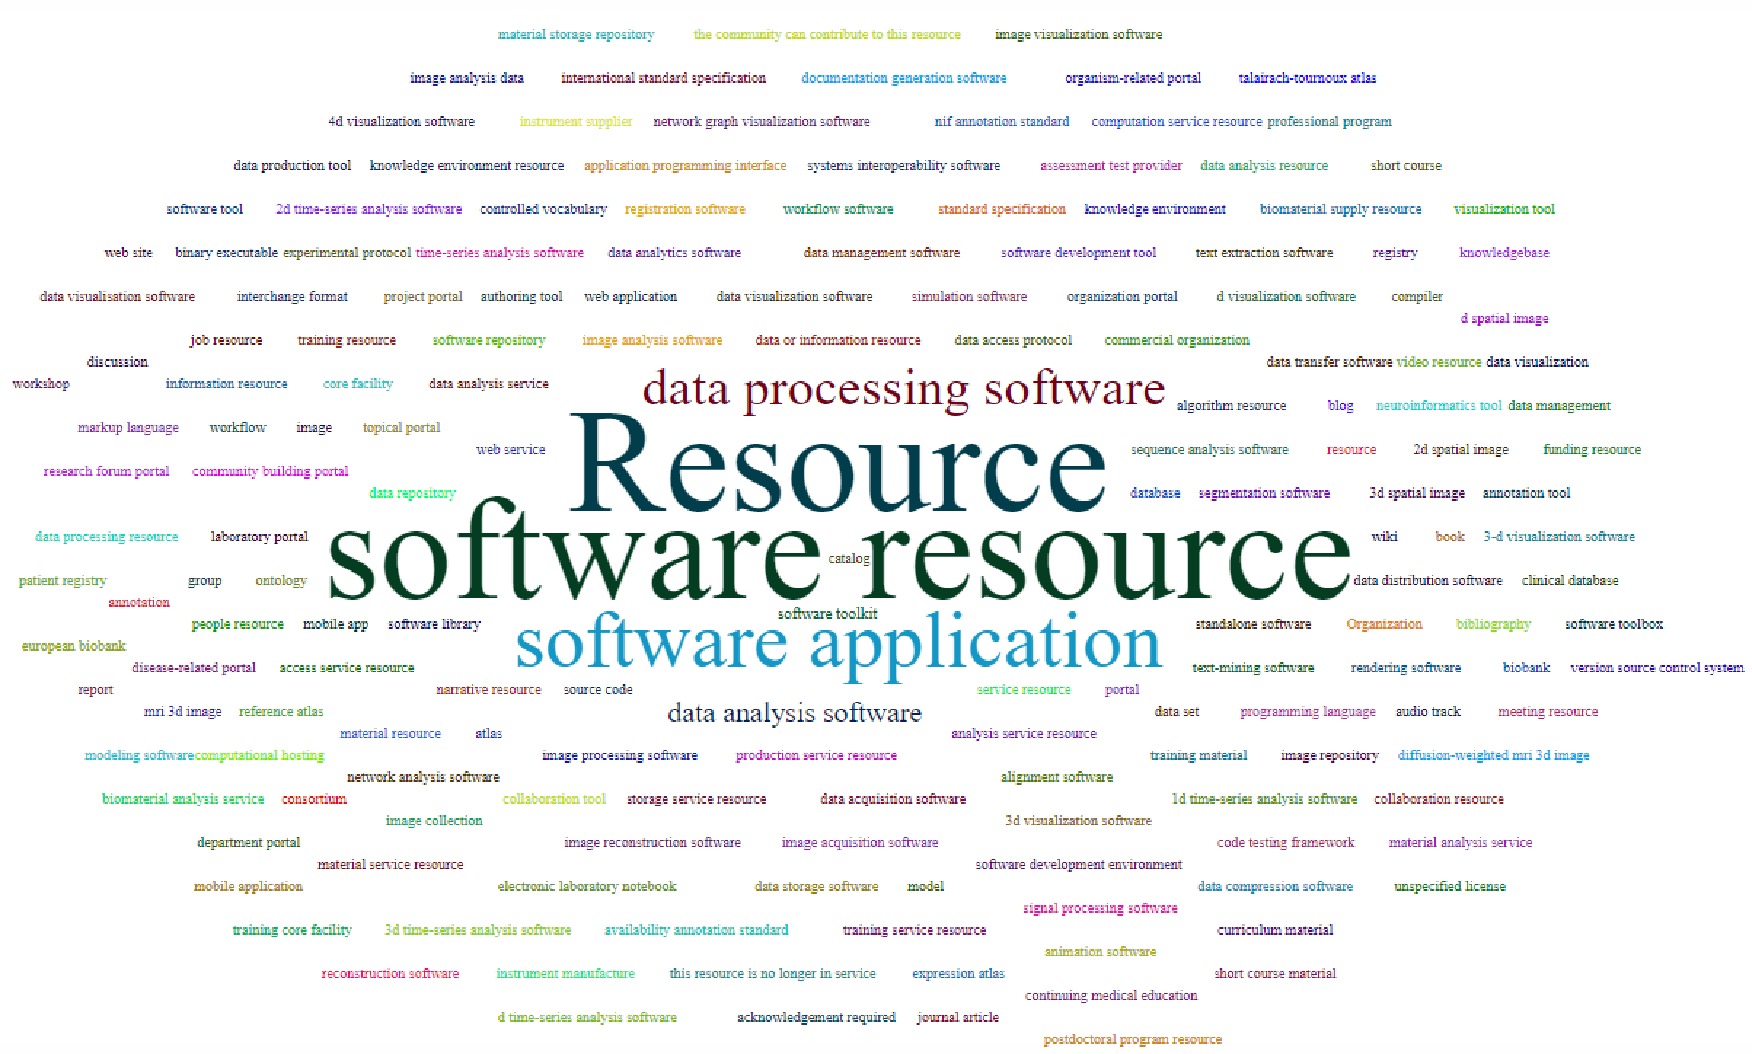
\includegraphics[width=1.2\textwidth]{4.graphics/figures/cloud}
	\caption{Word cloud of top 200 software types}
	\label{fig:chapter03:setup}
\end{figure}

After a manual analysis of the 200 of software types, generated from the word cloud, important software types that indicate possible software usage purpose has been identified. Sample of software types and their corresponding usage purpose is shown on the table below:

\begin{table}[h!]
	\begin{center}
		\caption{software types and potential purpose.}
		\label{tab:table1}
		\begin{tabular}{|l|l|} % <-- Changed to S here.
			\hline
			\textbf{Software Type} & \textbf{Purpose} \\
			\hline
			- Data acquisition software, Image acquisition software  & - Data collection, Recording  \\
			\hline
			- Data / Image  / Sequence  / Network  Analysis software  & - Data Analysis  \\
			\hline
			- Text mining software  & - Data Analysis  \\
			\hline
			- Signal processing software  & - Data Analysis  \\
			\hline
			- Data / 3D Visualization software & - Data Visualization  \\
			\hline
			- Simulation software  & - Simulation  \\
			\hline
			- Alignment software  & - Data pre/post-processing \\
			\hline
			- Rendering software  & - Modeling  \\
			\hline
			-	Code testing framework   & - programming  \\
			\hline
		\end{tabular}
	\end{center}
\end{table}
%-----------------------------
\section{Software purposes in ontologies   }
%-----------------------------

Ontologies are controlled vocabularies that provide formal naming and definition of properties and relation between concepts, entities, data etc.  Ontologies  are specialized  to a specific subject matter and every academic discipline creates ontologies to organize data into useful knowledge \citep{enwiki:1060388948}. 
Effective knowledge representation begins with analysis of ontologies with in the domain of interest \citep{chandrasekaran1999ontologies}. Accordingly, analysis of software ontologies have been done to find out possible software usage purposes. The software ontologies, that has been analyzed on this project are: WikiData, DBpedia, SWO (the software ontology), OntoSoft and codemeta.  
%-----------------------------
\subsection{Wikidata   }
%-----------------------------
Wikidata is a multilingual knowledge graph that is curated collaboratively by a Wikimedia community and serves as a freely available common source of structured data for everyone \citep{enwiki:1060114687, enwiki:1060408581}. 
Wikidata was created by Wikimedia foundation mainly to store meta data that can be used for other Wikimedia projects such as Wikipedia. Interestingly, wikidata is allowed to contain inconsistent and contradicting facts in order to embrace the diversity of knowledge about a given entity \citep{vrandevcic2012wikidata}. 

Although wikidata has a tremendous amount of data in it, there was no information that would indicate software usage purposes, rather information about software categories was found. Therefore, an indirect approach has been taken to list down possible software purposes from software categories by assuming each software category has essentially a software purpose associated to it. 

Wikidata comes with a bunch of tools like, SPARQL end point, query builder, data visualization tools, etc. Thus a SPARQL end point has bee utilized  to query a list software and their potential categories \emph{Take a look at the SPARQL query used on the Appendix}. 

Over 400 software categories have been found from the Query. To find out potential relation between these categories and to select more general software categories, a network analysis has been done using Gephi software.  Using Gephi software, clustering of related software categories and filtering has been made to have a more generalized software categories.

The procedure for network analysis has been described as follows:

\begin{itemize}
	\item First query result from the SPARQL terminal of wikidata has been downloaded in a csv file format. 
	\item Then, the csv file has been opened with Gephi software (version 0.9.2) as \emph{“undirected graph”}. This renders a network graph with overlapping nodes and edges. 
	\item To unravel the overlapping nodes for visibility, the lay-out of the graph is then changed to \emph{“Fruchterman Reingold”}. 
	\item To find out possible clusters from the network, from the list of statistical tools, \emph{“Modularity”} has been run. Then partition of nodes and edges has been done using \emph{“Modularity class”}. 
	\item Then to adjust size of nodes based on importance, node size ranking has been done with a \emph{“Degree”} parameter with \{minimum, maximum\} size of  \{20, 80\} respectively. 
	\item Then to select the most prominent nodes, among filter tool \emph{“Degree range”} filter has been used. The Degree range filter estimated prominence of the nodes between values of \{1, 60\} where the maximum value indicates the most prominent node. 
\end{itemize}


\begin{figure}[h]
	\myfloatalign
	\subfloat[Degree \{1-60\}]{
		\label{fig:chapter03:subfloat:grafik1}
		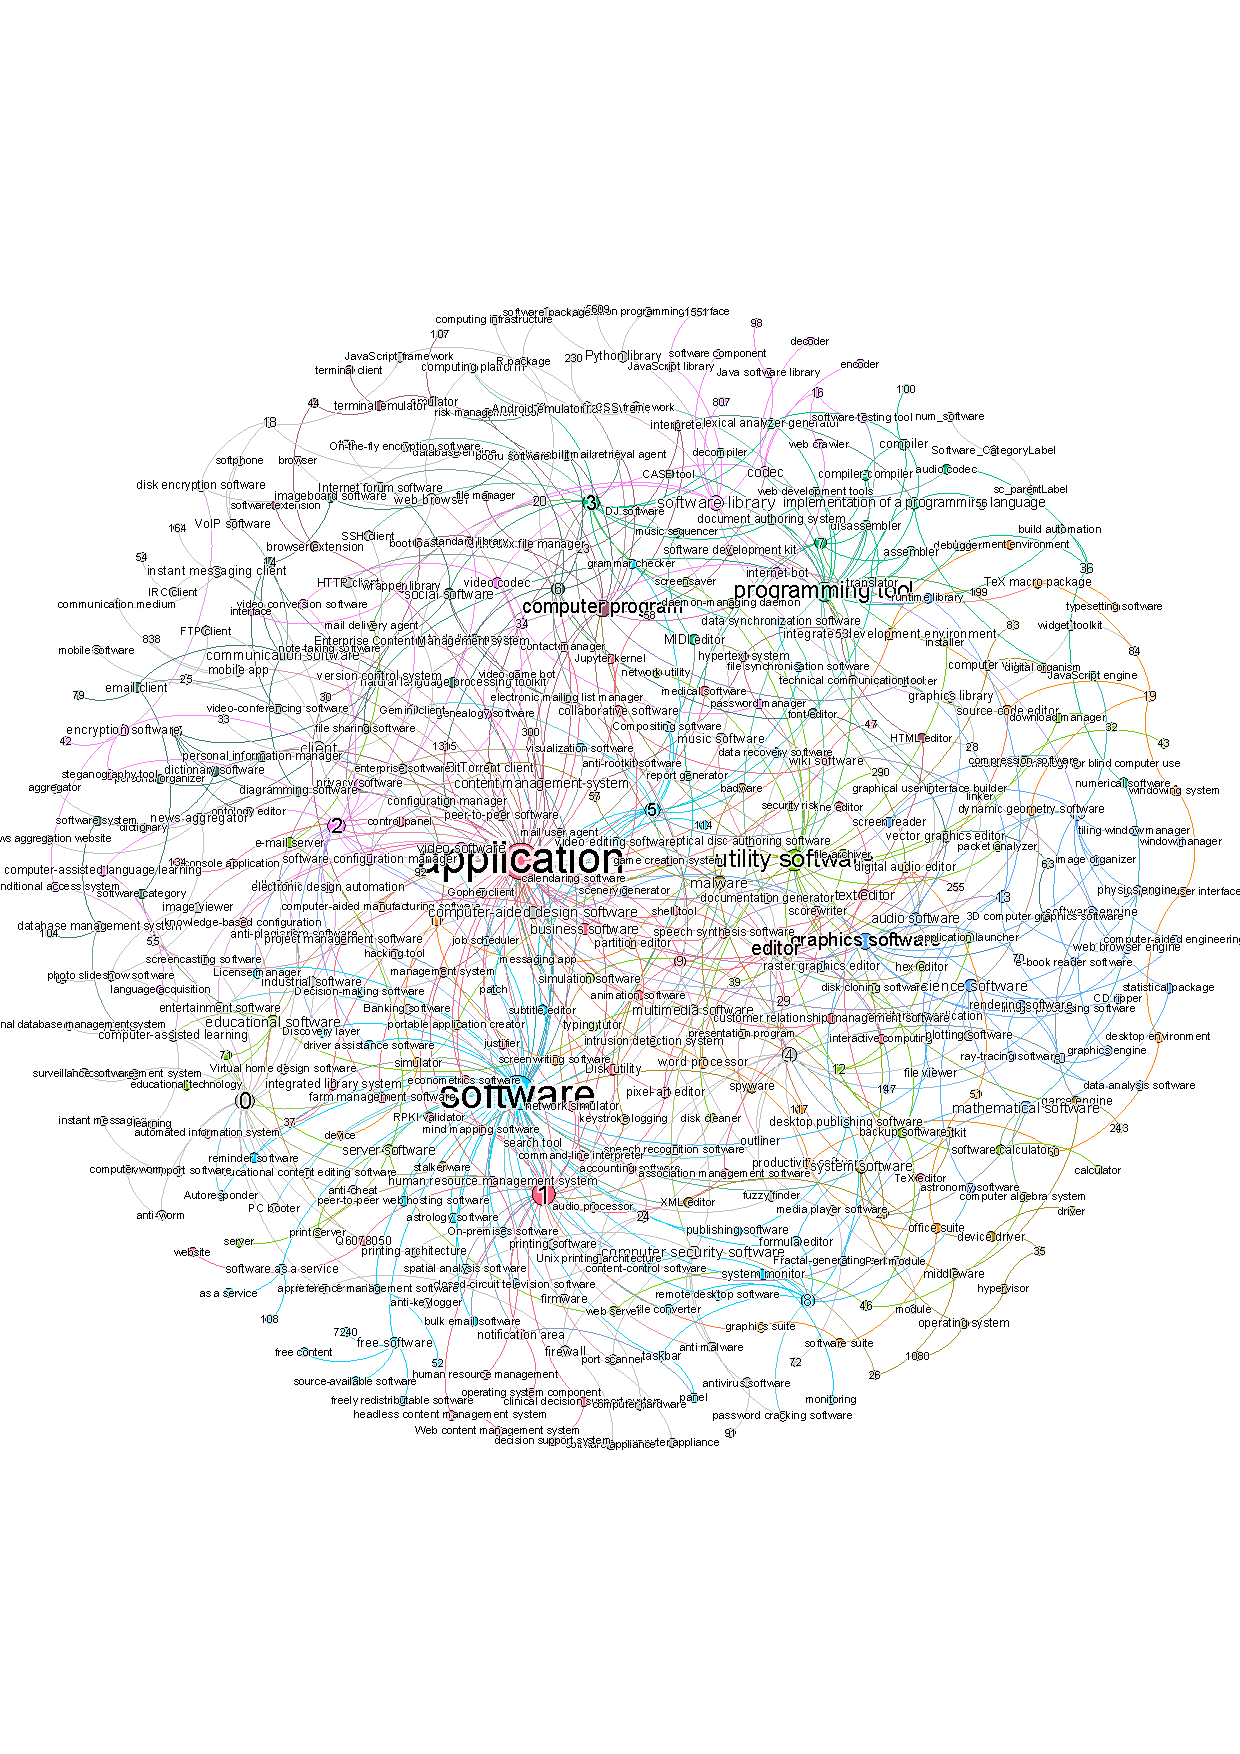
\includegraphics[width=.41\linewidth]{4.graphics/figures/Network1}
	} \quad
	\subfloat[Degree \{3-60\}.] {
		\label{fig:chapter03:subfloat:grafik2}
		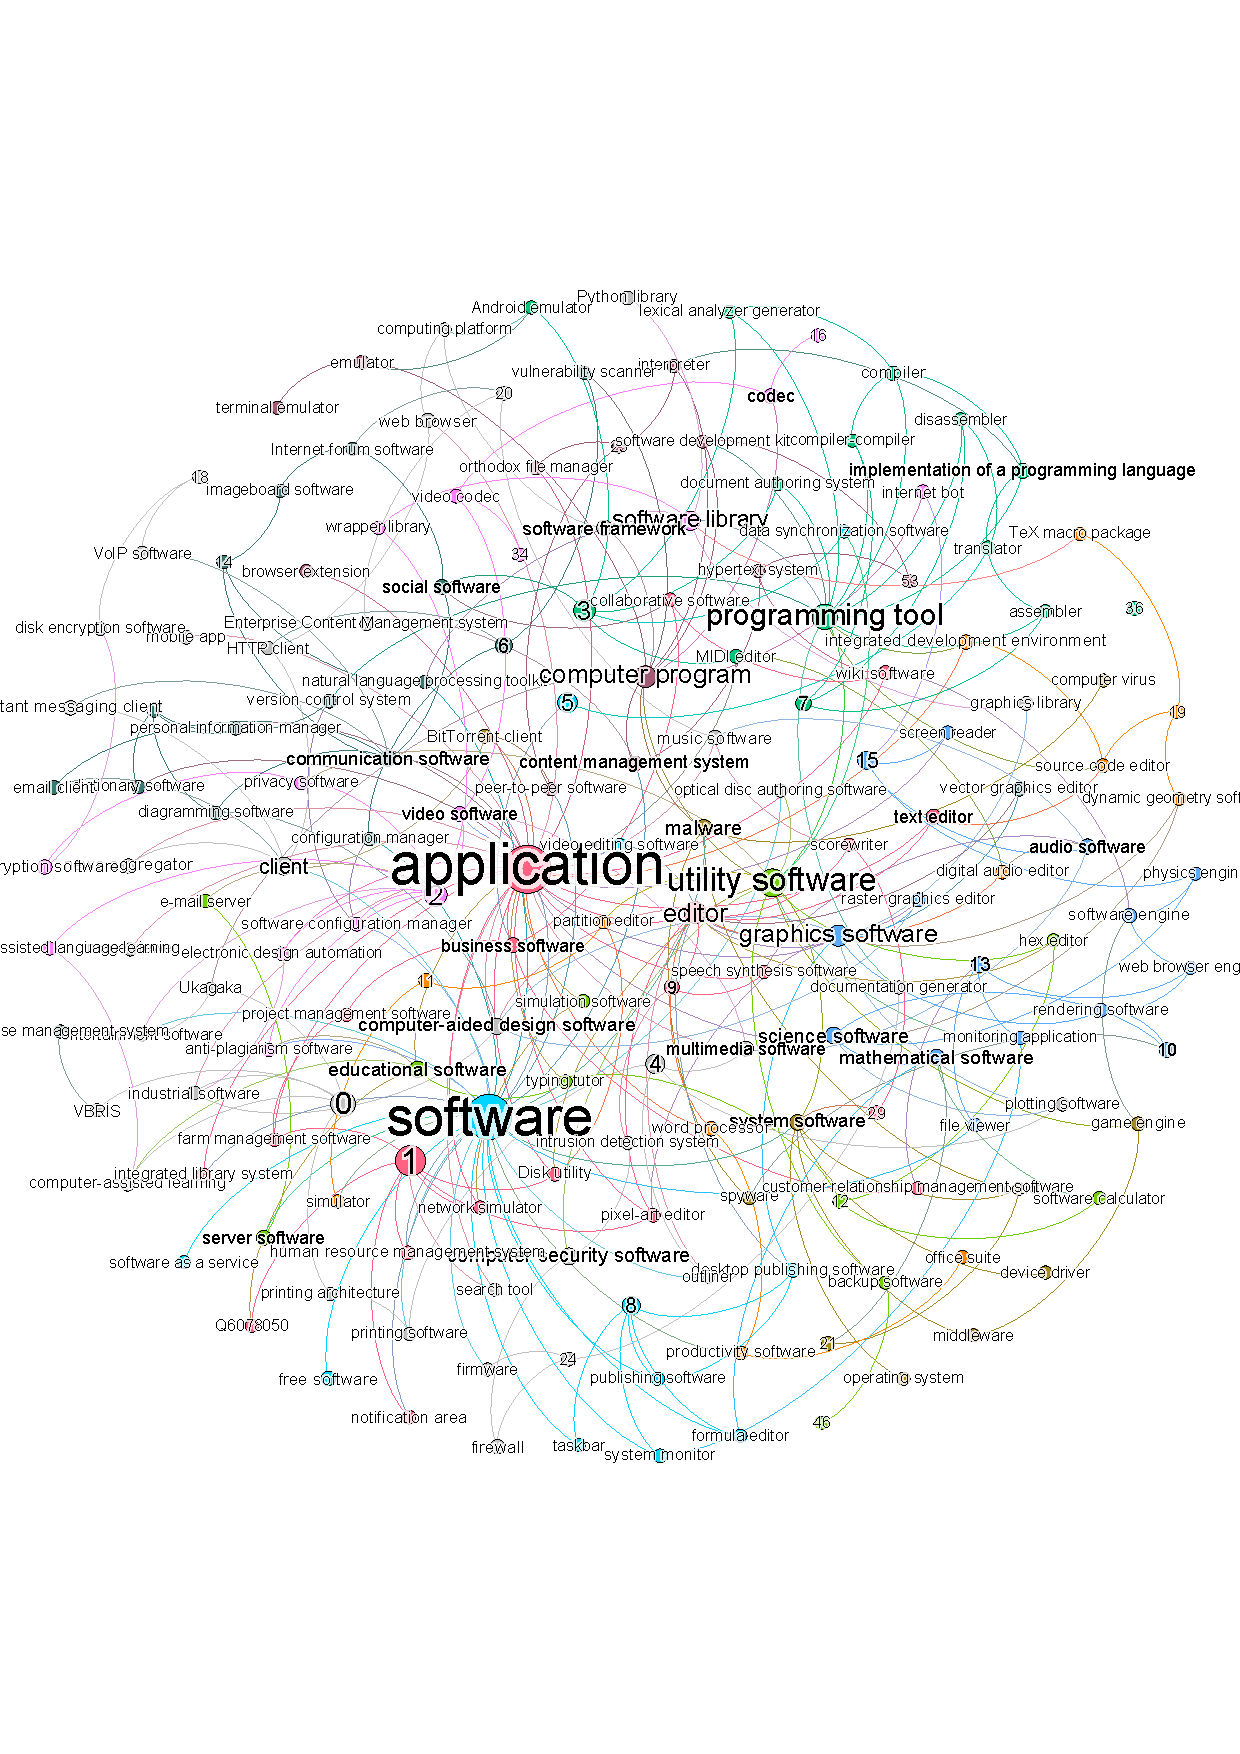
\includegraphics[width=.41\linewidth]{4.graphics/figures/Network2}
	} \\

\end{figure}
\begin{figure}[h]
	\myfloatalign
	\subfloat[Degree \{5-60\}]{
	\label{fig:chapter03:subfloat:grafik3}
	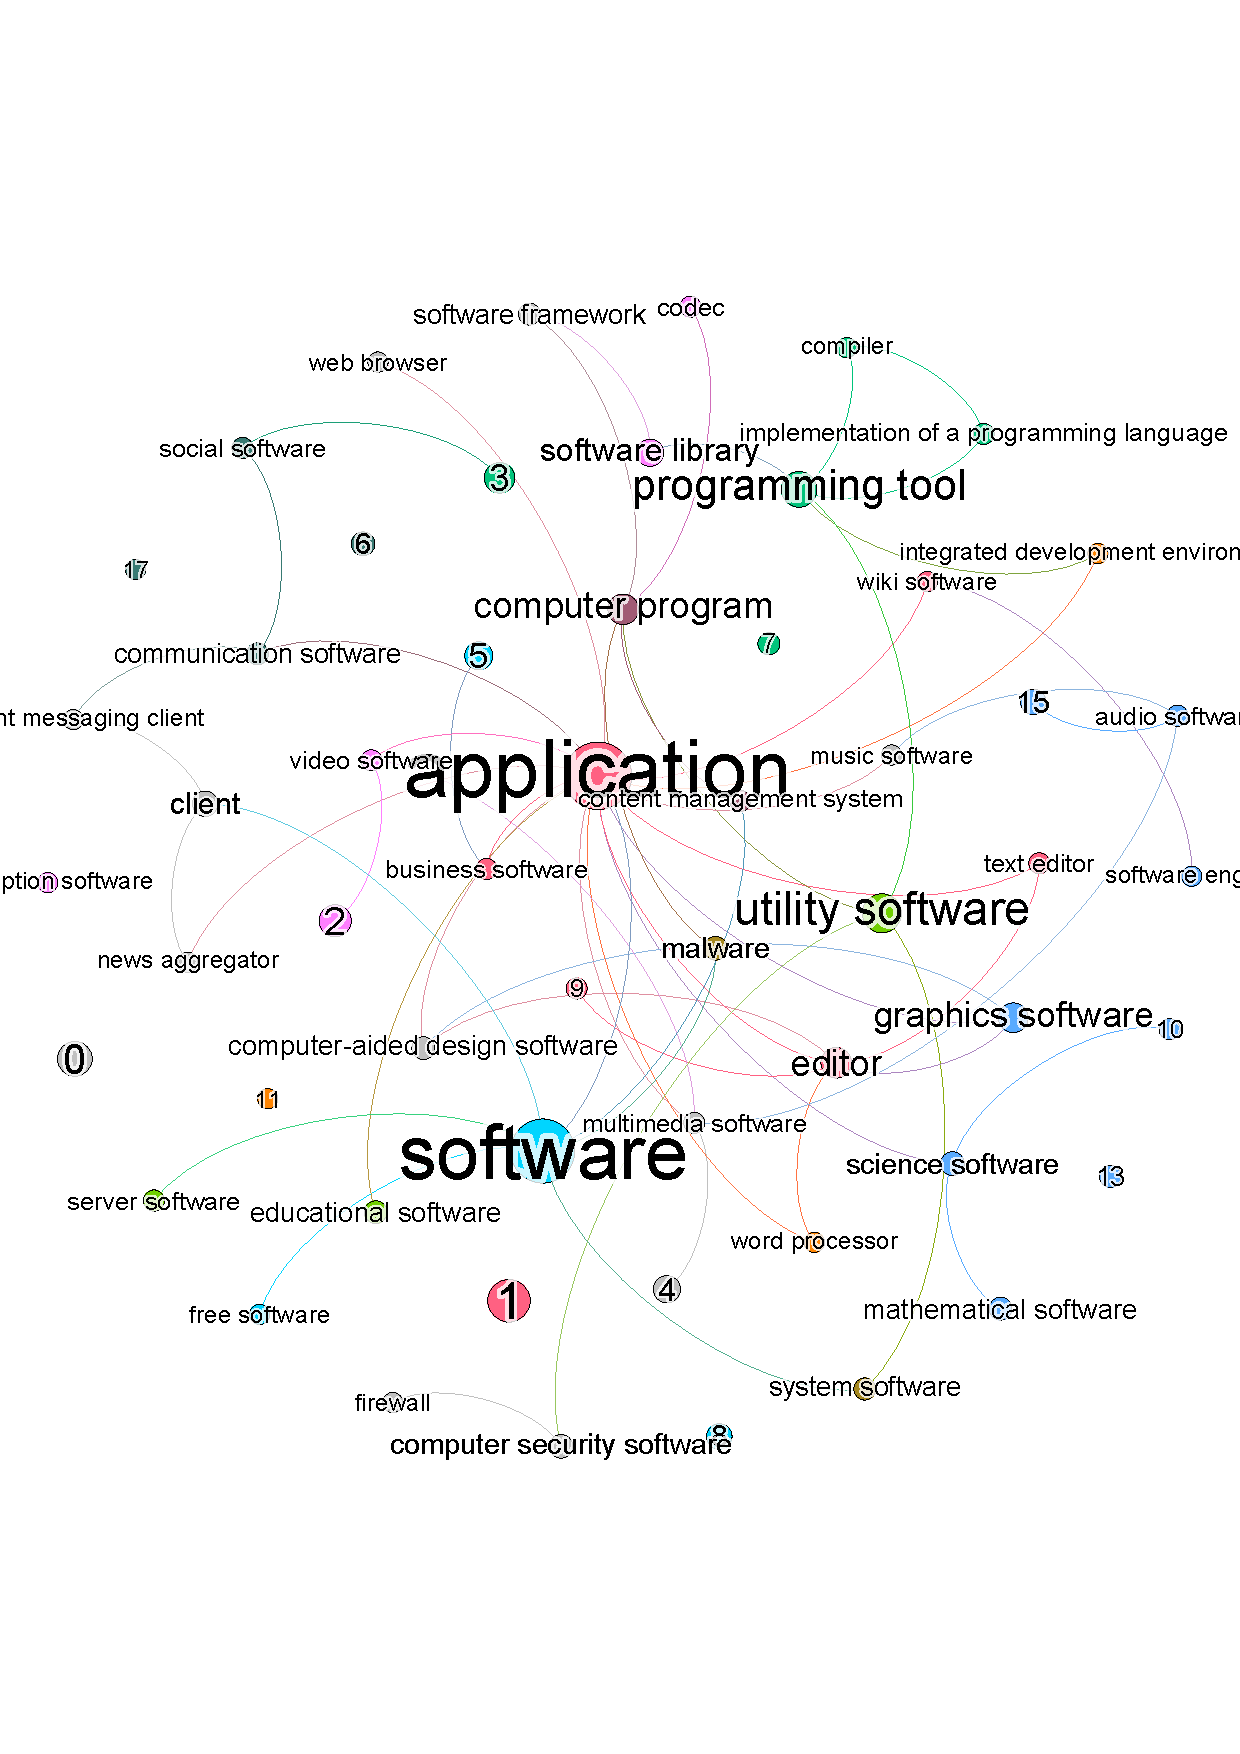
\includegraphics[width=.32\linewidth]{4.graphics/figures/Network3}
	} \quad
	\subfloat[Degree \{7-60\}]{
		\label{fig:chapter03:subfloat:grafik4}
		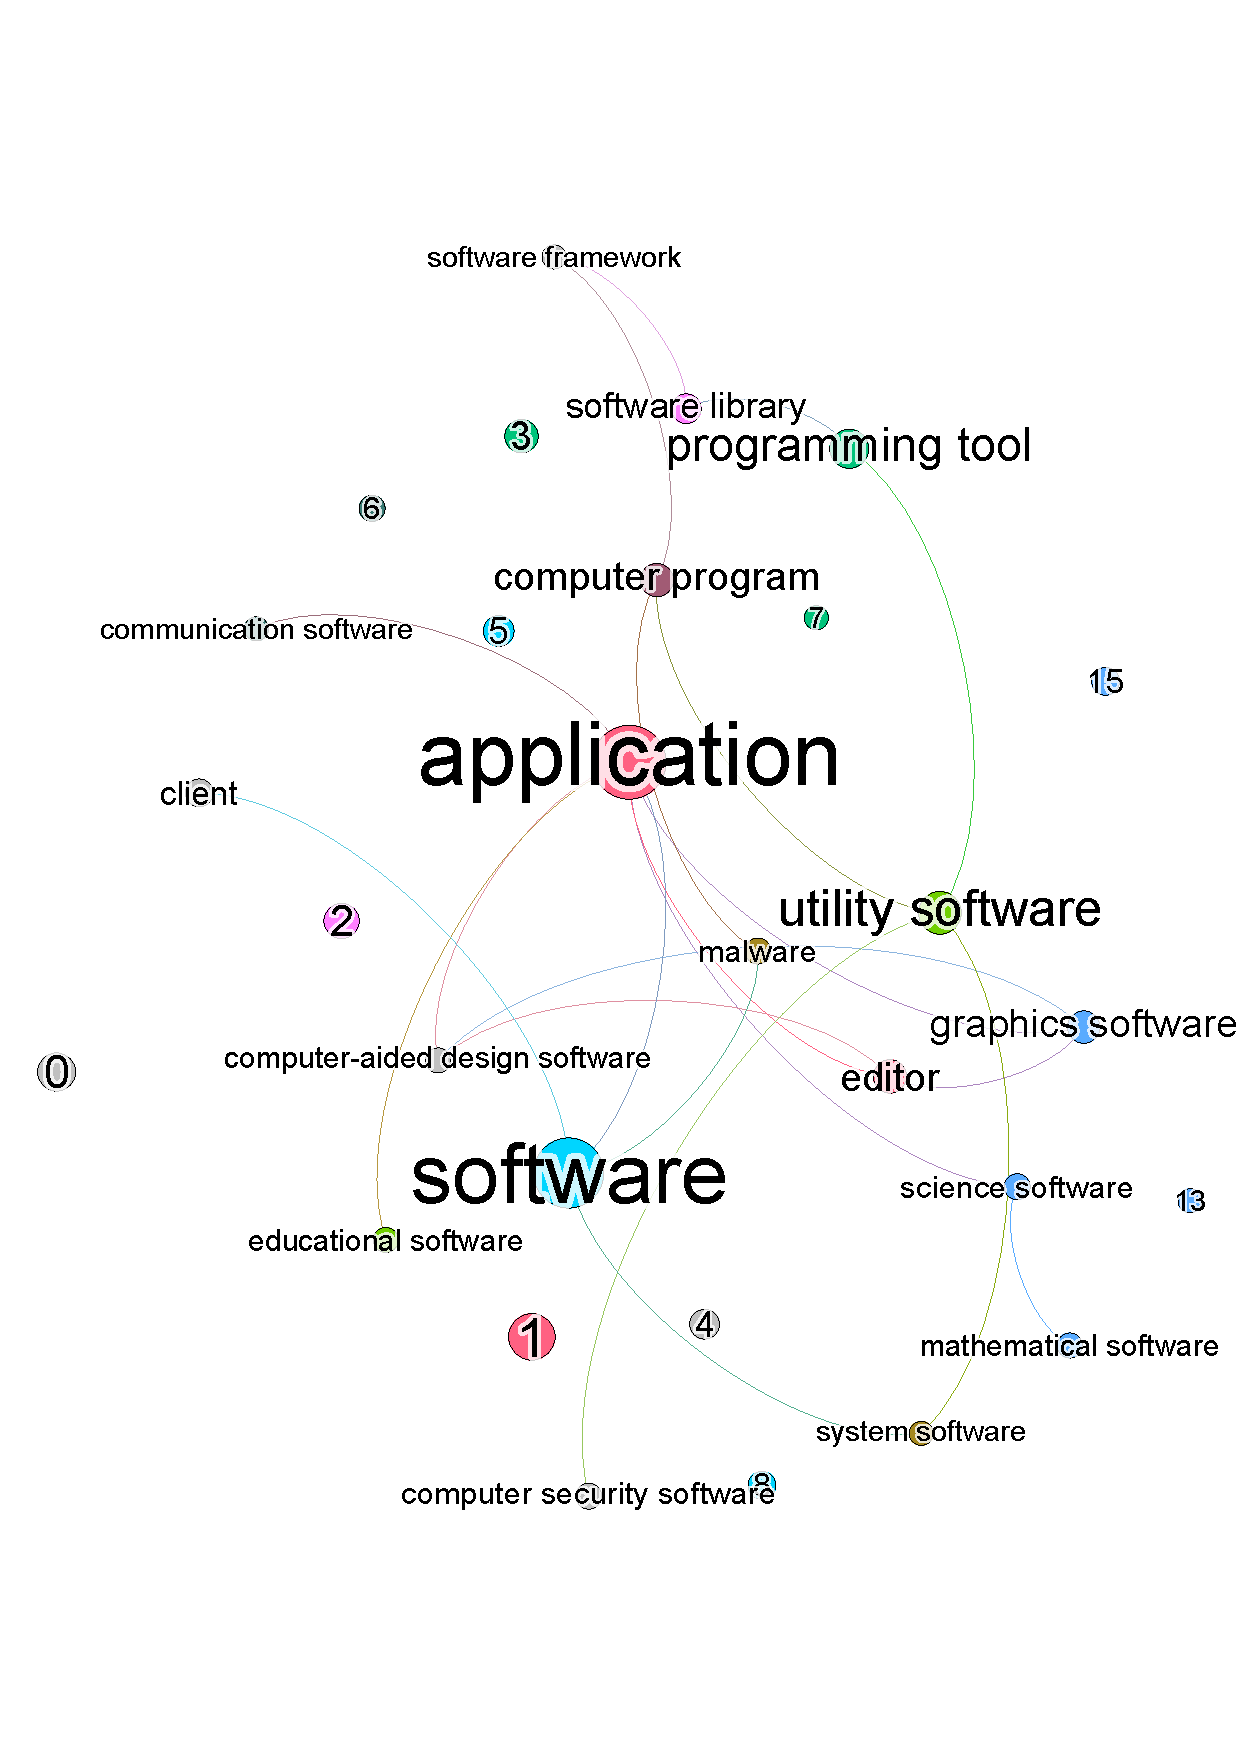
\includegraphics[width=.32\linewidth]{4.graphics/figures/Network4}
	}
	\caption[Subfloat - Figure]{Network analysis - prominent nodes of software categories in Wikidata.}
	\label{fig:chapter03:subfloat}
\end{figure}

According to the network analysis, major types of software categories are:

Numbered list 

\begin{table}[h!]
	\begin{center}
		\caption{Main types of software categories in wikidata.}
		\label{tab:table1}
		\begin{tabular}{|l|l|} % <-- Changed to S here.
			
			%\textbf{Value 1} & \textbf{Value 2} \\
			\hline
			- Application softwares & -	Utility software  \\
			- Computer security software & - System software \\
			- Measurements   & - Densitometric analysis \\
			- Client       & - Programming tool   \\
			- Software Library        & - Software framework  \\
			- Editor  & - Science software     \\
			- Graphics software     & - Computer aided design software \\
			- Mathematical software          & - Communication software \\
			\hline
		\end{tabular}
	\end{center}
\end{table}

The above software categories are related to each other as well. According to a manual analysis of wikidata, mathematical software, for instance, is subclass of science software and science software is subclass of application software. By analyzing the relation between the above software categories, overall three main types of software categories have been identified as follows:

\begin{enumerate}
 \item Application software 
 \item System software 
 \item Software Component 

\end{enumerate}

A simplified version of relation between software catefories is depicted on the grapgh below. 

\begin{figure}[htbp]
	\centering
	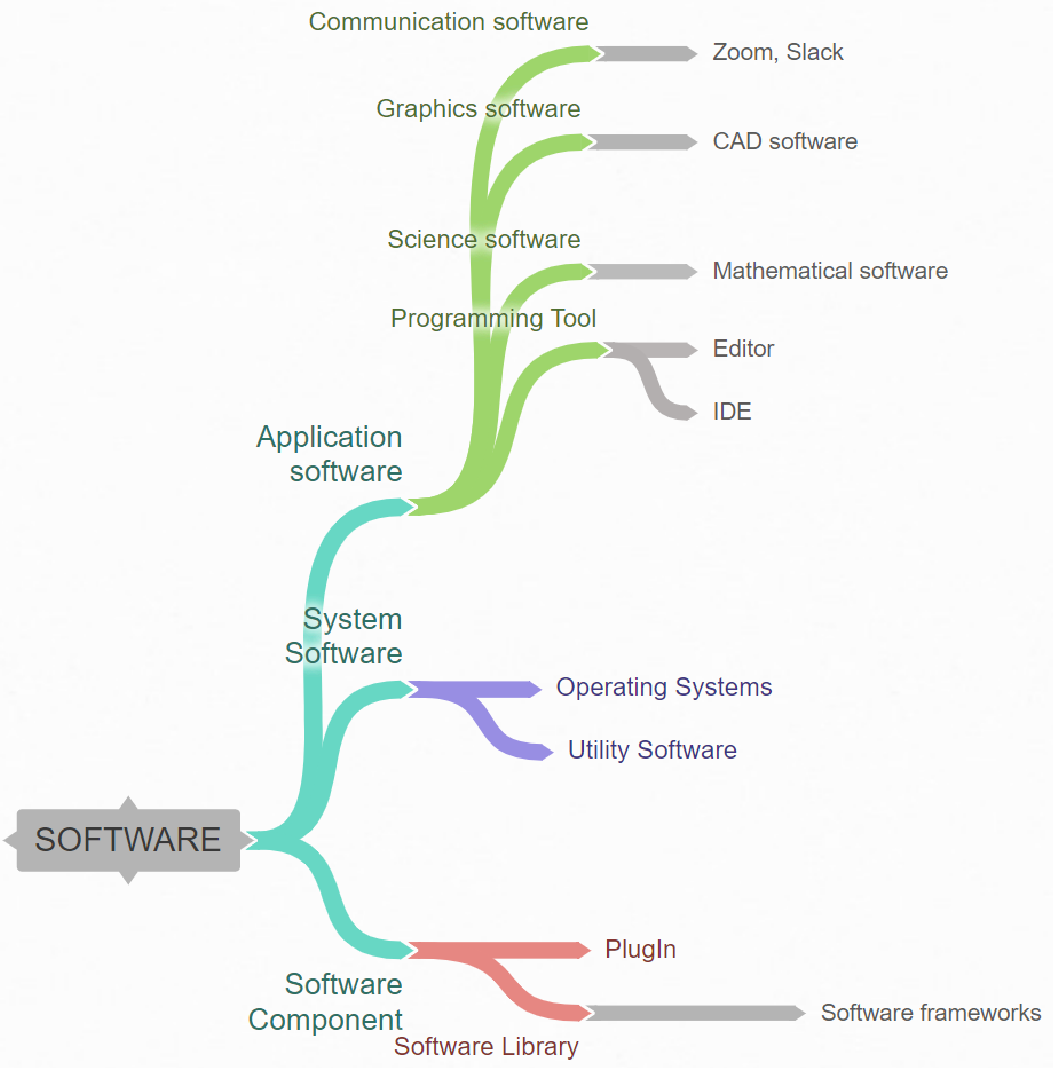
\includegraphics[width=1\textwidth]{4.graphics/figures/chart}
	\caption{Relation between main software categories in WikiData}
	\label{fig:chapter03:setup}
\end{figure}


%-----------------------------
\subsubsection{Identifying software purpose    }
%-----------------------------

The main aim of software category analysis of wikidata was to find possible software usage purposes from each software category. It is simple to define a software purpose when the software is used to carry out a specific task. 
According to Wikipedia, an application software is a  computer program that is designed to carry out a specific task other than operation of a computer and typically made for end-users \citep{enwiki:1060918552}. Most of research software can be considered as an application software, since they are used for a specific purpose. 

However it is worth mentioning that, there are two types of application software: horizontal (market) application software and vertical (market) application software. A horizontal (market) software is a kind of application software that is more generic, used in wide range of industries, and lack very specific purpose \citep{enwiki:1034388659}.  Examples of such types of software are word processors, spreadsheets, calendar applications, etc. On the other hand there are Vertical (market) application software whose purpose is to address needs of a specific niche in a business, research, or even a specific department within an organization \citep{enwiki:879502666}. Since we are trying to find purpose of a software, our main focus will be on application software that has specific purpose of use and used directly in a research process.  

Sub categories of application software with their respective purpose from Wikipedia and internet resources are have been gathered and summarized on the following table. 


Enumerate alpahbet

\begin{aenumerate}
	\item
	\item

\end{aenumerate}

Cite author and its paper as  Asia \citeauthor{bentley:1999} \citep{bentley:1999} 

Description

\begin{description}
  \item[Description-Label Test:] 
  \item[Description-Label Test:] 
\end{description}

%
% Section: Pictures
%
\section{Pictures}
\label{sec:chapter03:Pictures}
Insert pictures like this ...

\subsection{Simple picture}
\label{sec:chapter03:grafiken:simple}

%% inserting a picture

\begin{figure}[htbp]
 \centering
 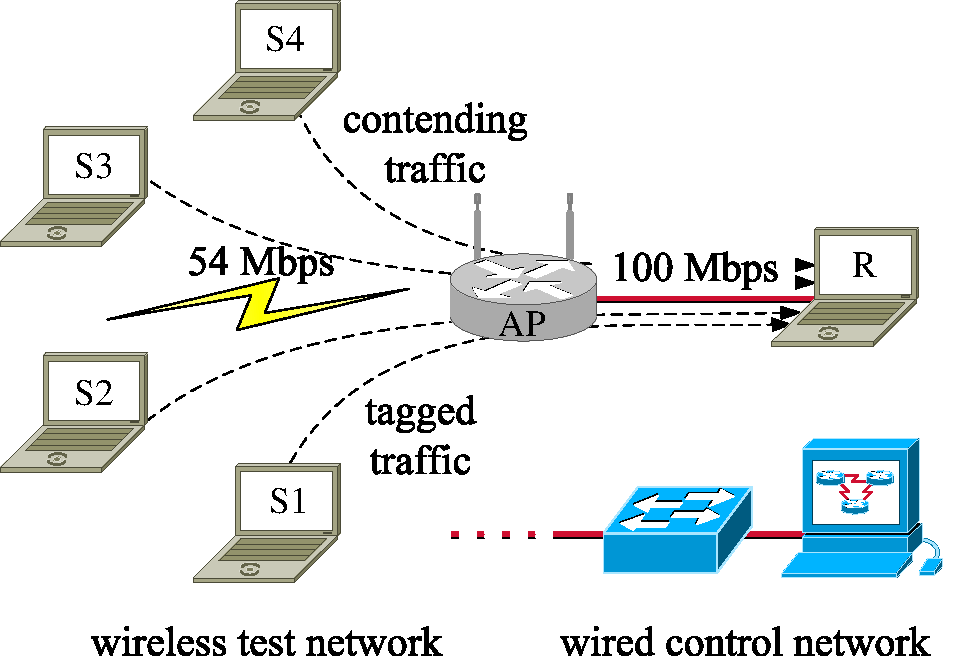
\includegraphics[width=0.5\textwidth]{4.graphics/figures/setup}
 \caption{Dies ist eine einfache Grafik}
 \label{fig:chapter03:setup}
\end{figure}



\subsection{Inserting a picture with sub-parts}
\label{sec:chapter03:grafiken:subfloat}

Insert a collection of pictures as shown here




\subsection{Two pictures side by side}
\label{sec:chapter03:grafiken:minipage}
Insert two pics like this ...

\begin{figure}[htbp]
  \centering
  \begin{minipage}[b]{5 cm}
    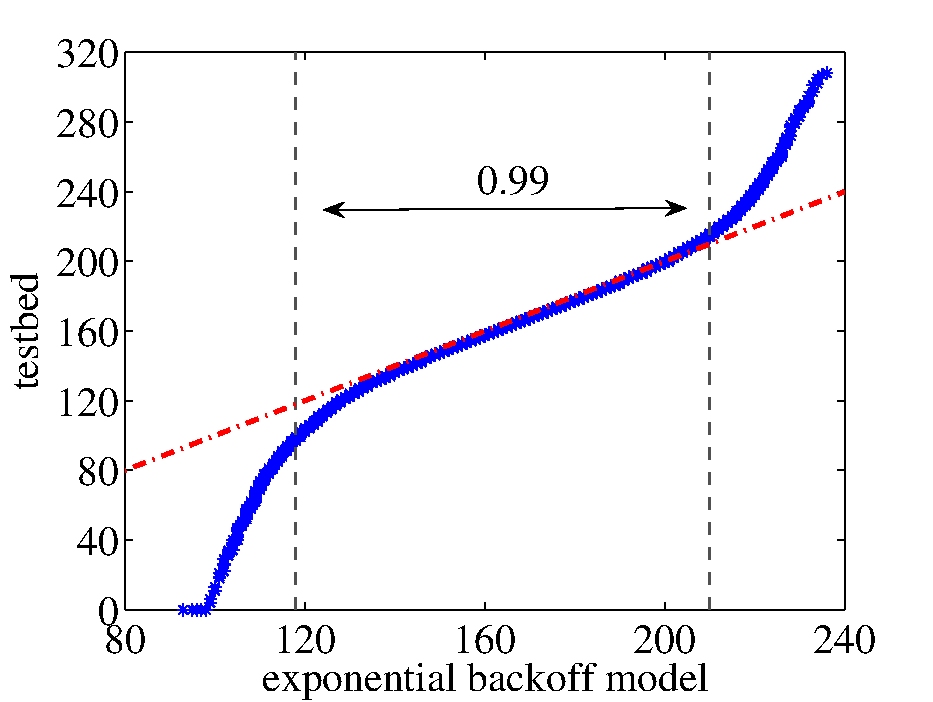
\includegraphics[width=\linewidth]{4.graphics/figures/qq-plot_gaus_vs_160} 
    \caption{Minipage-Grafik Nummero uno}
    \label{fig:chapter03:minipage:grafik1}
  \end{minipage}
  \begin{minipage}[b]{5 cm}
    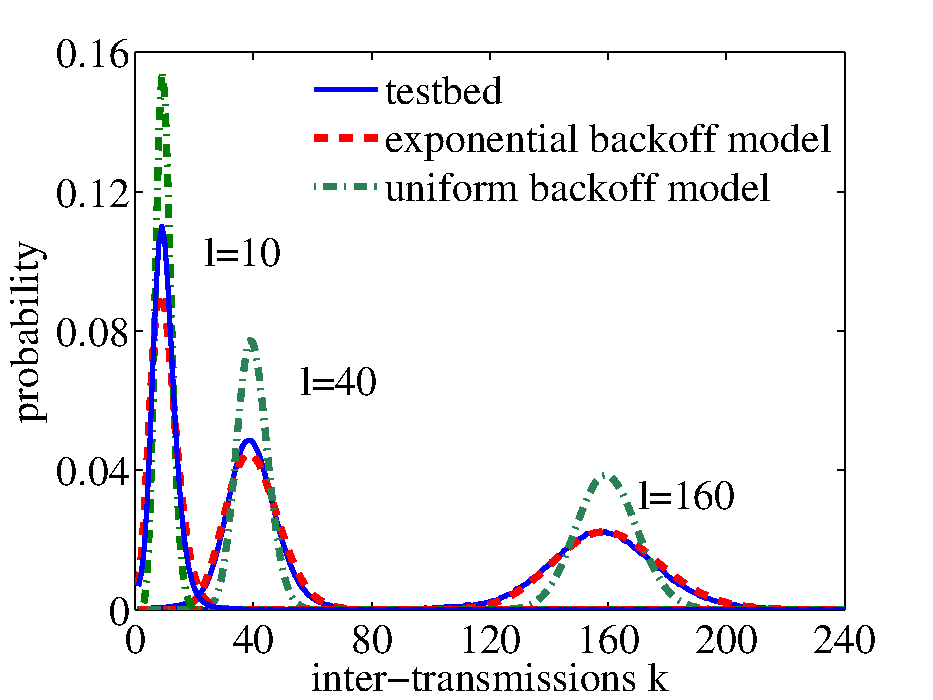
\includegraphics[width=\linewidth]{4.graphics/figures/pdf_gaus_vs_uni_vs_10_40_160}  
    \caption{Minipage-Grafik Nummer zwei}
    \label{fig:chapter03:minipage:grafik2}
  \end{minipage}
\end{figure}



%
% Section: Tabellen 
%
\section{Tables}
\label{sec:chapter03:tables}
Sed lobortis vestibulum euismod. Vivamus vestibulum gravida nisi vitae condimentum. Nullam 

%
% Section: Listings 
%
\section{Listings}
\label{sec:chapter03:listings}
Aliquam ut pretium lectus. Curabitur in eros et sapien aliquet luctus ut sit amet eros. Proin et libero non mi venenatis aliquet at sed lorem. 


%
% Section: Equations
%
\section{Equations}
\label{sec:chapter03:equations}
Pellentesque sed quam quis dui vulputate convallis ut ac diam. In hac habitasse platea dictumst. 
%
\begin{equation}
 U = R * I
\end{equation}

 Aenean quis commodo libero. Nulla quis semper dolor.
%
\begin{equation}
 I = \frac{U}{R} 
\end{equation}

In the following we use probability theory to derive closed-form expressions for the fairness that is achieved among $M$ contending stations. We tag station $M$ and denote $K_i$ the inter-transmissions of station $i = 1 \dots M-1$ and let $K = \sum_{i=1}^{M-1} K_i$. The conditional probability $P[K\!=\!k|l]$ can be defined for $M \ge 2$ as
%
\begin{equation}
\mathsf{P}[K\!=\!k|l] = \mathsf{P} \Biggl[\sum_{i=1}^{M-1} K_i = k \Big| l \Biggr]
\label{eq:chapter03:exactpmf}
\end{equation}
%
where the random variables $K_i$ are the integers that satisfy
%
\begin{equation*}
\sum_{j=1}^{K_i} b_i(j) \le \sum_{j=1}^{l} b_M(j) \;\;\; \textmd{and} \;\;\; \sum_{j=1}^{K_i+1} b_i(j) > \sum_{j=1}^{l} b_M(j) .
\end{equation*}


%
% Section: Theorem and Proof
%
\section{Theorem and Proof}
\label{sec:chapter03:theorem}
We use the central limit theorem to derive the long-term fairness. In the sequel, we denote normal random variables $N(\mu,\sigma^2)$ where $\mu$ is the mean and $\sigma^2$ the variance.
%
\begin{Theorem}[Gaussian approximation]
\label{th:chapter03:twostationsgaussian}
%
Let the $b_i(j)$ be i.i.d. random variables with mean $\mu$ and variance $\sigma^2$ and let $M=2$. For $k,l \gg 1$ (\ref{eq:chapter03:exactpmf}) is approximately Gaussian where
%
\begin{equation*}
\mathsf{P}[K \!\le\! k|l] \approx \mathsf{P}\biggl[ N(0,1) \le \frac{\mu\,(k-l)}{\sigma\,\sqrt{k+l}} \biggr] .
\end{equation*}
%
\end{Theorem}
%
\begin{proof}
%
For $M=2$ we have from (\ref{eq:chapter03:exactpmf}) that
%
\begin{equation*}
\mathsf{P}[K \!<\! k|l] = \mathsf{P} \Biggl[\, \sum_{j=1}^k b_1(j) > \sum_{j=1}^l b_2(j) \Biggr]
\end{equation*}
%
and after expansion and some normalization this equals
%
\begin{equation*}
= \mathsf{P}\Biggl[ \frac{\sum_{j=1}^{l}b_2(j) - l\mu}{\sigma\sqrt{l}} - \frac{\sum_{j=1}^{k}b_1(j) - k\mu}{\sigma\sqrt{l}} < \frac{\mu(k-l)}{\sigma\sqrt{l}} \Biggr].
\end{equation*}
%
Using the central limit theorem it follows that
%
\begin{equation*}
\mathsf{P}[K \!<\! k|l] \approx \mathsf{P} \biggl[ N(0,1) - N \biggl(0,\frac{k}{l}\biggr) < \frac{\mu(k-l)}{\sigma\sqrt{l}} \biggr] .
\end{equation*}
%
Since the normal distribution with zero mean is symmetric we can replace the subtraction of $N(0,k/l)$ by addition. Furthermore, the sum of two normal random variables $N(\mu_1, \sigma_1^2)$ and $N(\mu_2, \sigma_2^2)$ is normal with $N(\mu_1+\mu_2, \sigma_1^2+ \sigma_2^2)$ such that
%
\begin{equation*}
\mathsf{P}[K \!<\! k|l] \approx \mathsf{P} \biggl[ N\biggl(0,\frac{k+l}{l}\biggr) < \frac{\mu(k-l)}{\sigma\sqrt{l}} \biggr] .
\end{equation*}
%
Finally, we use that if $X$ is $N(a\mu,a^2\sigma^2)$ then $Y = X/a$ is $N(\mu,\sigma^2)$ with $a^2 = (k+l)/l$ to standardize the result.
%
\end{proof}

Th. \ref{th:chapter03:twostationsgaussian} assumes i.i.d. random countdown values. It does, however, not make any assumption about their distribution.
